%Kelompok Memory Allocation (2)
%Arjun Yuda Firwanda
%Dezha Aidil Martha
%Dwi Septiani Tsaniyah
%Muh.Rifky Prananda
%Yusuf Al-Qordhawi

Putty

\section {Membahas Tentang "Putty"}

\subsection {A. Memahami Putty}

Putty adalah program open source yang dapat digunakan untuk melewati protokol jaringan SSH (Secure Shel), Telnet dan Rlogin. Protokol ini dapat digunakan untuk remote pada komputer melalui jaringan, baik LAN (Local Area Network) atau internet. Program ini digunakan oleh pengguna komputer saat ini, sekarang untuk menghubungkan, mensimulasikan, dan masalah yang terkait dengan jaringan. Program ini tentu saja juga sebagai sebuah terowongan (enkapsulasi atau pembungkusan protokol) di dalam jaringan.
Protokol dapat digunakan untuk mengetahui jaringan atau menjalankan sesi jarak jauh di komputer.

\begin{enumerate}

	\item SSH (Secure Shell)
	Merupakan protokol jaringan yang memungkinkan pertukaran data melalui saluran aman antara dua perangkat jaringan.

	\item Rlogin
	Sistem yang memungkinkan kita dapat masuk dari satu sistem ke sistem lain tanpa kata sandi tambahan.

	\item Telnet
	Adalah jaringan telekomunikasi yang digunakan di Internet atau Local Area Network (LAN) untuk menyediakan fasilitas komunikasi berbasis teks yang menggunakan koneksi terminal virtual.

\end{enumerate}


\subsection {Mengetahui Lebih dalam Putty}

PuTTY adalah alat komunikasi antara pengguna dengan server yang dipergunakan oleh pemilik server untuk berkomunikasi dengan server mereka atau server lain dengan menggunakan perintah teks yang berguna untuk menjalankan perintah tertentu. Artinya dengan perintah teks si pemilik server dapat berkomunikasi dengan servernya tanpa ada kendala dalam konfigurasi dengan system.

"PuTTY adalah klien SSH dan telnet, yang dikembangkan awalnya oleh Simon Tatham untuk platform Windows PuTTY adalah perangkat lunak open source yang tersedia dengan kode sumber dan dikembangkan dan didukung oleh sekelompok relawan.
- www.putty.org "

Tujuan utama PuTTY adalah menjadi aplikasi multi-platform (aplikasi yang bisa dijalankan diOperating System apa saja) yang mampu menjalankan sistem operasi. Dan Ia juga dapat disebut terminal xterm (emulator).

Jendela utama PuTTY memiliki sesi yang berjalan di komputer jarak jauh dan dapat mengirim perintah langsung ke komputer jarak jauh, melalui konfigurasi system. Artinya dengan alat ini dapat dijalankan dengan jarak jauh melalui konfigurasi dengan system.

PuTTY memberikan beberapa keunggulan yang berbeda, terutama dari jarak jauh. Lebih mudah untuk mengalami. Pada saat yang sama memfasilitasi pengembang untuk mengembangkan aplikasi yang sesuai dengan kebutuhan sistem saat ini. 

\begin{figure}[ht]
\centerline{
\includegraphics[width=1\textwidth]{figures/puttyexe.jpg}}
\caption{gambar putty.}
\label{putty}
\end{figure}


\subsection {Pengertian SSH(Secure Shell)}

Menurut pendapat \cite{Jusuf.Heni2015Penggunaan Secure Shell} SSH adalah suatu kriptografi yang digunakan untuk mengkomunikasikan data yang ada pada perangkat jaringannya untuk membuatnya lebih aman lagi. Dalam konsep menggunkan SSH ini harus di dukung oleh suatu server atau di dalam computer. Pada akun SSH ini dirancang untuk digunakan sebagai pola piker Telnet dan shell pada jarak jauh yang tidak aman, yang mengirimkan suatu informasi terutama pada kata sandinya dalam bentuk yang sederhanan dan mudah untuk disadap. Enkripsi disediakan oleh SSH untuk memberikan suatu kerahasiaan dan integritas data melalui jaringan tidak aman seperti internet.

\begin{figure}[ht]
\centerline{\includegraphics[width=1\textwidth]{figures/ssh.gif}}
\caption{gambar ssh.}
\label{ssh}
\end{figure}

 
\subsection {Pengertian Rlogin (Remote Login)}

Rlogin atau Remote Login merupakan salah satu dari berbagai macam layanan internet yang memungkinkan pengguna internet untuk mengakases (masuk)  sebuah host dalam lingkup jaringan internet, seorang user dapat mengoperasikan sebuah host dari jarak jauh tanpa harus kontak secara fisik dengan host. Di sana user dapat melakukan maintenance atau pemeliharaan, menjalankan sebuah program, bahkan menginstall program baru di host.

\begin{figure}[ht]
\centerline{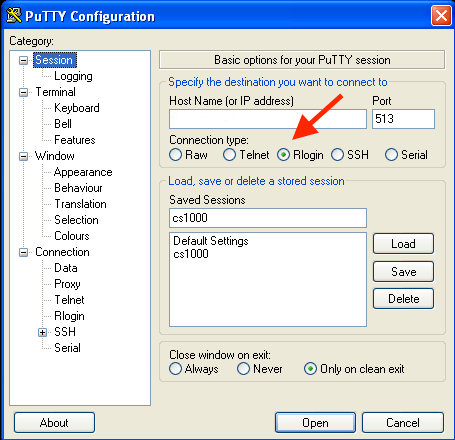
\includegraphics[width=1\textwidth]{figures/rlogin.png}}
\caption{gambar rlogin.}
\label{rlogin}
\end{figure}
